\documentclass[11pt]{article}

\usepackage[spanish,activeacute]{babel}
\usepackage{titlesec}
\usepackage{graphicx}
\usepackage{subcaption}
\usepackage{float}
\usepackage[bottom]{footmisc}
\usepackage[hidelinks]{hyperref}


\setlength{\parindent}{1.0em}
\setlength{\parskip}{1.0em}
\setlength{\emergencystretch}{5.0em}
\titlespacing*{\section}{0em}{3.5em}{1.5em}
\setcounter{tocdepth}{1}
\hypersetup{
	linktoc=all
}


\title{\Huge Software en formato fuente}
\author{Eugenia Damonte, Ariel Fideleff y Mart\'in Go\~ni}
\date{}


\begin{document}
	\pagenumbering{gobble}
	\maketitle
	\newpage
	\tableofcontents
	\newpage
	\pagenumbering{arabic}
	
	
	\section{Configuraci\'on previa}
		Antes de comenzar a resolver los ejercicios configuramos \texttt{vim} para editar archivos en C. Para hacer esto abrimos el archivo \texttt{\textasciitilde/.vimrc} (en todo caso de no existir, hay que crearlo) que es el archivo de configuraci'on de \texttt{vim}. Estaba vac'io por lo que le le a'nad'imos dos l'ineas: \texttt{set nocp} y \texttt{filetype plugin on}. Lo que hace el primer comando es desactivar el modo de compatibilidad. 'Este hace que algunas de las funciones de \texttt{vim} sean deshabilitadas o modificadas para que se comporte de manera similar a \texttt{vi}, el antecesor de \texttt{vim}. La segunda permite utlizar el plugin \texttt{filetype}.
		
		Luego para asegurarnos de tener todos los paquetes de \texttt{vim} utlizamos el comando \texttt{sudo apt-get install vim-gui-common vim-runtime}. El primer paquete tuvo que instalarse demorando varios minutos por la velocidad de descarga abismal de los repositorios. El segundo, por el otro lado ya estaba instalado en nuestro caso.
		
		Finalmente creamos el archivo de configuraci'on para los archivos con extensi'on \texttt{.c}, llamado \texttt{c.vim}. Para poder crearlo primero tuvimos que crear la carpeta \texttt{\textasciitilde/.vim/ftplugin}, que es donde se ponen los archivos de configuraci'on. Luego abrimos el mismo con \texttt{vim} y escribimos las configuraciones que quer'iamos usar.
		
		\begin{figure}[H]
			\centering
			\begin{subfigure}[b!]{0.7\linewidth}
				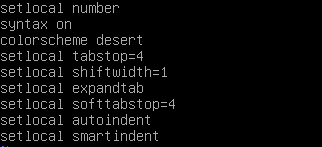
\includegraphics[width=\linewidth]{Images/Preamble/Preamble.PNG}
				\caption*{Las configuraciones para los archivos \texttt{.c}.}
			\end{subfigure}
		\end{figure}
		
		
	\section{Uso b'asico de gcc}
		Antes de comenzar con el proyecto en si decidimos asegurarnos de que \texttt{gcc} funcionaba correctamente y que sab'iamos usarlo. Para hacer esto copiamos el programa de ejemplo, \texttt{circulo.c}, que se encuentra en el apunte provisto.
		
		\begin{figure}[H]
			\centering
			\begin{subfigure}[b!]{0.7\linewidth}
				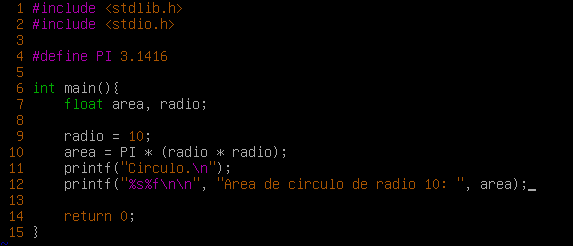
\includegraphics[width=\linewidth]{Images/Seccion 1/S1.PNG}
				\caption*{El programa de ejemplo \texttt{circulo.c}.}
			\end{subfigure}
		\end{figure}
		
	\subsection{Compilaci'on directa}
		Una vez copiado el programa realizamos una compilaci'on directa para asegurarnos de que el programa funcionase correctamente. Para hacer esto usamos el comando \texttt{gcc -o circulo circulo.c}. Lo que hace el argumento \texttt{-o} es especificar como se debe llamar el archivo de salida, si no se usa el archivo se nombra \texttt{a.out}.
		
		\begin{figure}[H]
			\centering
			\begin{subfigure}[b!]{0.7\linewidth}
				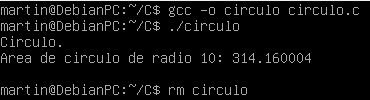
\includegraphics[width=\linewidth]{Images/Seccion 1/S1 parte dos.PNG}
				\caption*{Muestra de funcionamiento de \texttt{circulo.c}.}
			\end{subfigure}
		\end{figure}
		
	\subsection{Compilaci'on compleja}
		Habiendo comprobado que \texttt{gcc} funcionaba correctamente decidimos intentar compilar el mismo archivo, \texttt{circulo.c}, de manera compleja. Es decir haciendo cada uno de los pasos que realiza el compilador a la hora de transformar un archivo en C en un programa ejecutable.
	
	\subsection{Compilaci'on compleja - Preprocesamiento}
		 El preprocesado es la primera etapa de modificaci'on del c'odigo fuente. Sirve para que en la fase de compilaci'on, que es la siguiente, el compilador pueda leer correctamente el c'odigo. 

   		 %pueden observar que mi léxico está formado por 3 palabras (y una de ellas es "léxico")
    
    		El trabajo del preprocesador consiste en llevar a cabo las instrucciones dadas por las \texttt{directivas de preprocesador} (que, en el caso de C y C++, son las que comienzan con un numeral, como \#define, \#include, \#ifdef y \#error).

   		En el archivo \texttt{circulo.c} podemos encontrar la directiva  ``\#define PI 3.1416'', que declara %no sé si está bien decir "declarar" acá
    una constante de nombre  ``PI'' y valor 3.1416. Esta constante es llamada en la funci'on \texttt{main} de manera que, en vez de escribir  ``3.1416'', escribimos simplemente  ``PI''.

	    	En la figura \ref{}, %buenoyasaben
    		se observa el c'odigo preprocesado -que obtuvimos como salida del comando \texttt{gcc -E circulo.c}-. Si prestamos atenci'on, la directiva antes mencionada no figura en esta salida. Adem'as, en la l'inea que en el c'odigo fuente dec'ia \texttt{''area = PI * (radio * radio)''}, ahora dice \texttt{''area = 3.1416 * (radio * radio)''}. 

   		En resumen, lo que hizo el preprocesador fue tomar esa definici'on que le indicamos en la directiva y pegar el valor de la constante en las partes del c'odigo en donde se hac'ia referencia a ella.

	\subsection{Compilaci'on compleja - Compilaci'on}
		El primer paso es la compilaci'on donde se transforma el c'odigo en C a assembler del procesador de la computadora. Para hacer esto usamos el comando \texttt{gcc -S circulo.c}. Luego verificamos que haya funcionado mostrando las primeras l'ineas del archivo \texttt{circulo.s}, que es donde \texttt{gcc} almacena el archivo en assembler.

		\begin{figure}[H]
			\centering
			\begin{subfigure}[b!]{0.7\linewidth}
				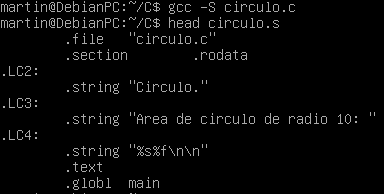
\includegraphics[width=\linewidth]{Images/Seccion 1/S1 parte tres.PNG}
				\caption*{El primer paso, la compilaci'on}
			\end{subfigure}
		\end{figure}
		
	\subsection{Compilaci'on compleja - Ensamblado}
		Una vez compilado procedimos a ensamblar el archivo. Es decir transformar el archivo en assembler a c'odigo objeto, un archivo binario en lenguaje m'aquina. Hicimos esto con el comando \texttt{as -o circulo.o circulo.s}. Luego verificamos que haya funcionado revisando que tipo de archivo era \texttt{circulo.o}.
		\begin{figure}[H]
			\centering
			\begin{subfigure}[b!]{0.7\linewidth}
				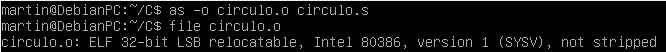
\includegraphics[width=\linewidth]{Images/Seccion 1/S1 parte cuatro.PNG}
				\caption*{El segundo paso, el ensamblado.}
			\end{subfigure}
		\end{figure}
		
	\subsection{Compilaci'on compleja - Enlazado}
		Finalmente enlazamos el archivo, en este paso es donde nos encontramos con problemas. El comando que se da en el apunte no funciona. Al usarlo da varios errores indicando que las librerias usadas como argumentos no existen, as'i como algunas de las opciones.
	
		\begin{figure}[H]
			\centering
			\begin{subfigure}[b!]{0.7\linewidth}
				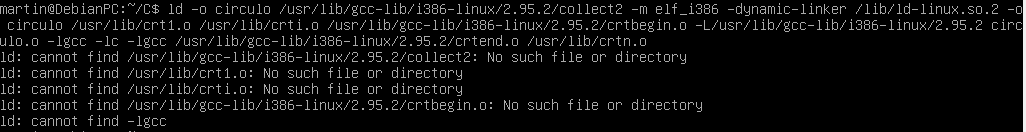
\includegraphics[width=\linewidth]{Images/Seccion 1/S1 parte cinco.PNG}
				\caption*{El primer intento de usar \texttt{ld}, siguiendo el apunte.}
			\end{subfigure}
		\end{figure}
		
		Dado todos los errores que hab'ia decidimos borrar todas las opciones innecesarias y probar nuevamente. Al hacer esto los errores anteriores desaparecieron pero uno nuevo apareci'o, este dec'ia ``\texttt{cannot find entry symbol \textunderscore\/start}''. Esto se traduce como ``\texttt{no se encuentra el simbolo de entrada \textunderscore\/start}. Luego de algo de investigaci'on descubrimos que este error se debe a que el verdadero punto de entrada\footnotemark\/ de un programa es \texttt{\textunderscore\/start}, no \texttt{main}, \texttt{\textunderscore\/start} simplemente redirige a 'el. Para solucionar esto usamos el argumento \texttt{--entry main} para especificar la funci'on \texttt{main} como el punto de entrada del programa.
		
		Una vez hechos estos cambios la funci'on no daba mas errores y el programa parecia estar listo para usar. A la hora de ejecutarlo, sin embargo este no era reconocido como un programa ejecutable. Para asegurarnos de haber hecho todo correctamente revisamos que el archivo existiese as'i como tambi'en sus permisos, siendo estos correctos.
		
		\footnotetext{El punto de entrada de un programa es donde se ejecutan las primeras instrucciones y se pasa control al programa.}
		
		\begin{figure}[H]
			\centering
			\begin{subfigure}[b!]{0.7\linewidth}
				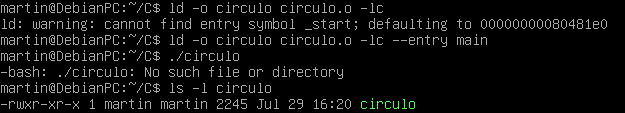
\includegraphics[width=\linewidth]{Images/Seccion 1/S1 parte seis.PNG}
				\caption*{El segundo intento de usar \texttt{ld}.}
			\end{subfigure}
		\end{figure}
		
		Dado que no pod'iamos ejecutar el programa decidimos intentar volver a a'nadir algunas de las opciones que no causaban errores. Primero volvimos a a'nadir las opciones \texttt{-m elf\textunderscore\/i386} y \texttt{-dynamic-linker /lib/ld-linux.so.2}. La primera opci'on define el objetivo del compilador\footnotemark. La segunda define la ubicaci'on del enlazador din'amico\footnotemark\/ a usar.
		
		\footnotetext[2]{El objetivo del compilador es lo que determina que tipo de c'odigo objeto debe producir la funci'on.}
		\footnotetext{Un enlazador din'amico o \textit{dynamic linker} es una forma de enlazar los archivos binarios que se necesitan para que el programa funcione. En este caso el c'odigo de las funciones se mantiene en la biblioteca y la hora de ejecutar el programa se cargan en memoria.}
		
		Luego de hacer estos cambios logramos ejecutar el programa, que parec'ia funcionar correctamente. Sin embargo al final de este tuvimos el error \texttt{Segmentation fault}. Para tratar de averiguar de donde ven'ia el error decidimos debuggear el programa utilizando \texttt{gdb}.
		
		\begin{figure}[H]
			\centering
			\begin{subfigure}[b!]{0.7\linewidth}
				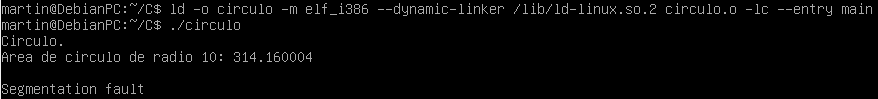
\includegraphics[width=\linewidth]{Images/Seccion 1/S1 parte siete.PNG}
				\caption*{El tercer intento de usar \texttt{ld}.}
			\end{subfigure}
			\begin{subfigure}[b!]{0.7\linewidth}
				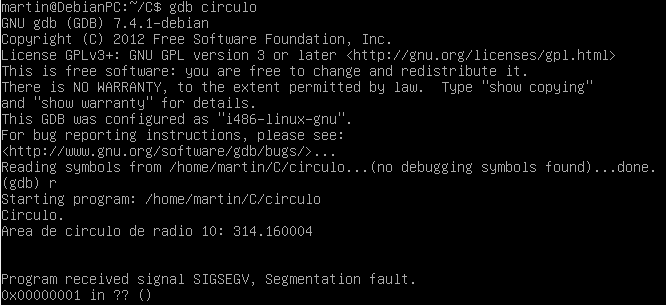
\includegraphics[width=\linewidth]{Images/Seccion 1/S1 parte ocho.PNG}
				\caption*{Nuestro intento de debuggear el programa.}
			\end{subfigure}
		\end{figure}
		
		Cuando intentamos debuggear el programa nos encontramos con algo extra'no, \texttt{gdb} no sab'ia de que l'inea proven'ia el error. Esto nos llev'o a creer que proven'ia de el enlazado del programa, y no del programa en si. Luego de buscar m'as todav'ia encontramos el problema, nos faltaba incluir las librer'ias que reqeria el enlazador din'amico. Para entender porque pasa esto hay que entender c’omo funciona el comando.
		
		Lo primero que hace el comando es especificar la ubicaci'on del enlazador din'amico que requieren las dem'as librer'ias para acceder a las funciones din'amicas de C. Luego se incluyen otras tres librer'ias \texttt{/usr/lib/i386-linux-gnu/crt1.o}, \texttt{/usr/lib/i386-linux-gnu/crti.o} y \texttt{/usr/lib/i386-linux-gnu/crtn.o}. La primera es la librer'ia que tiene referencias a los archivos que requiere el enlazador(\texttt{/lib/libc.so.6} y \texttt{/usr/lib/libc\textunderscore\/nonshared.a}). Las otras dos se encargan de que existan \texttt{\textunderscore\/init} y \texttt{\textunderscore\/fini}, que son el c'odigo de inicializaci'on y finalizaci'on. Algo importante de recordar es que la ubicaci'on de las librerias puede cambiar dependiendo del sistema y la instalaci'on especifica. En nuestro caso las encontramos buscando en \texttt{/usr/lib} y revisando todas las carpetas que parec'ian tener alguna relaci'on.
	
		Es importante notar la posici'on de las librer'ias, \texttt{crti.o} debe ir despu'es de \texttt{crt1.o}. Esto es porque este hace referencia al primero. Adem'as ambas deben ir antes de el archivo que se est’a enlazando. Finalmente \texttt{crtn.o} va al final del comando, despu'es de todos los dem'as argumentos.
		
		\begin{figure}[H]
			\centering
			\begin{subfigure}[b!]{0.7\linewidth}
				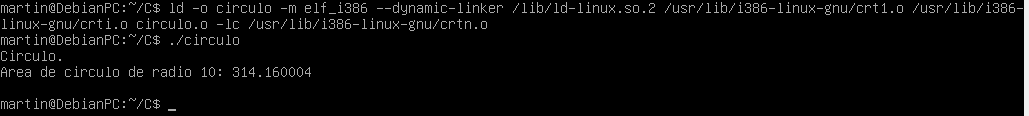
\includegraphics[width=\linewidth]{Images/Seccion 1/S1 parte nueve.PNG}
				\caption*{}
			\end{subfigure}
		\end{figure}
		
		Luego de hacer todo esto el programa finalmente funcion'o y se ejecut'o de manera correcta y sin errores. Habiendo terminado decidimos que ya ten'iamos el suficiente conocimiento para intentar compilar un programa usando \texttt{make}.
		
		
		
		


















%Remove whitspace when done, for ease of work.
\end{document}
